\documentclass[a4paper,12pt]{article}

        \usepackage{fontspec}
        \setmainfont{Times New Roman}
        \usepackage{polyglossia}
        \setdefaultlanguage{russian}
        \usepackage{amsmath,amssymb}
        \usepackage{upgreek}
        \usepackage{graphicx}
        \usepackage{float}
        \usepackage{array}
        \usepackage{geometry}
        \usepackage{ragged2e}
        \usepackage{setspace}
        \usepackage{caption}
        \usepackage{enumitem}

        \geometry{left=30mm,right=15mm,top=20mm,bottom=20mm}
        \setlength{\parindent}{1.25cm}
        \setlength{\parskip}{0pt}
        \onehalfspacing
        \setlength{\emergencystretch}{3em}
        \renewcommand{\arraystretch}{1}
        \setlength{\tabcolsep}{6pt}
        \captionsetup{font={normalsize},labelfont={bf},justification=centering}
        \graphicspath{{../../Results/Graphs/}{./}}

        % Греческие обозначения, указанные в требованиях, набираются прямым
        % шрифтом во всех формулах отчёта.
        \renewcommand{\alpha}{\upalpha}
        \renewcommand{\beta}{\upbeta}
        \renewcommand{\gamma}{\upgamma}
        \renewcommand{\delta}{\updelta}
        \renewcommand{\phi}{\upphi}
        \renewcommand{\varphi}{\upvarphi}
        \renewcommand{\epsilon}{\upepsilon}
        \renewcommand{\varepsilon}{\upvarepsilon}
        \renewcommand{\zeta}{\upzeta}
        \renewcommand{\sigma}{\upsigma}
        \renewcommand{\kappa}{\upkappa}

        \newcommand{\heading}[1]{%
          \par\noindent{\centering\fontsize{16pt}{24pt}\selectfont\bfseries #1\par}%
        }
        \newcommand{\tabletitle}[1]{\par\noindent\makebox[\textwidth][r]{#1}\par\noindent}
        \newcommand{\figurecaption}[1]{%
          \par\noindent{\centering #1\par}%
        }
        \newcommand{\mathtext}[1]{\text{#1}}

        \begin{document}
        \fontsize{14pt}{21pt}\selectfont
        \justifying
        % ragged2e меняет \parindent при включении выравнивания; задаём
        % требуемый отступ первой строки после \justifying.
        \setlength{\parindent}{1.25cm}
        \setlength{\parskip}{0pt}

        % Титульный лист: весь текст набран LaTeX; изменяется только ФИО студента.
        \begin{titlepage}
        \thispagestyle{empty}
        \begin{center}
        \begin{minipage}[t]{0.23\textwidth}
          \vspace{0pt}
\includegraphics[width=3.0cm]{bauman_logo.png}
        \end{minipage}\hfill
        \begin{minipage}[t]{0.72\textwidth}
          {\fontsize{12pt}{14pt}\selectfont
          \centering
          Министерство науки и высшего образования Российской Федерации\\
          Федеральное государственное автономное образовательное учреждение высшего образования\\
          «Московский государственный технический университет имени Н.Э. Баумана\\
          (национальный исследовательский университет)»\\
          (МГТУ им. Н.Э. Баумана)}
        \end{minipage}
        \end{center}
        \vspace{4mm}\hrule height 1.2pt\vspace{2mm}\hrule
        \vspace{8mm}
        {\fontsize{12}{14}\selectfont
        \noindent\begin{tabular}{@{}p{29mm}@{\hspace{6mm}}p{130mm}@{}}
        ФАКУЛЬТЕТ & \underline{\makebox[\linewidth][l]{«СПЕЦИАЛЬНОЕ МАШИНОСТРОЕНИЕ»}}\\[3mm]
        КАФЕДРА & \underline{\makebox[\linewidth][l]{«РАКЕТНЫЕ И ИМПУЛЬСНЫЕ СИСТЕМЫ» (СМ6)}}
        \end{tabular}}
        \vfill
        \begin{center}
          {\fontsize{25}{30}\selectfont\bfseries ОТЧЁТ}\\[10mm]
          {\fontsize{20}{25}\selectfont\bfseries ПО ЛАБОРАТОРНОЙ РАБОТЕ}\\[12mm]
          {\fontsize{18}{22}\selectfont\bfseries НА ТЕМУ:}\\[10mm]
          {\fontsize{18}{22}\selectfont\bfseries ИССЛЕДОВАНИЕ ВЛИЯНИЯ ПАРАМЕТРОВ}\\
          {\fontsize{18}{22}\selectfont\bfseries ЗАРЯДА ТВЁРДОГО ТОПЛИВА}
        \end{center}
        \vspace{10mm}
        \noindent\begin{tabular}{@{}p{40mm}p{54mm}p{62mm}@{}}
        Студент\hspace{4mm}\underline{СМ6-72} & \hfill\underline{\hspace{36mm}} & Барышев С.А.\\[-1mm]
        \hspace{17mm}(Группа) & \hfill(Подпись, дата) & \hfill(И.О. Фамилия)\\[10mm]
        Преподаватель & \hfill\underline{\hspace{36mm}} & Гудков И.А.\\[-1mm]
        \hspace{28mm} & \hfill(Подпись, дата) & \hfill(И.О. Фамилия)
        \end{tabular}
        \vfill
        \begin{center}2026 г.\end{center}
        \end{titlepage}

        \setcounter{page}{2}
        \heading{Содержание}
        \noindent\begin{tabular}{@{}p{0.88\textwidth}r@{}}
        Введение & 3\\
        1. Цель работы & 4\\
        2. Краткие теоретические сведения & 5\\
        3. Исходные данные & 7\\
        4. Результаты расчёта & 8\\
        5. Параметры для построения на миллиметровой бумаге & 12\\
        6. Заключение & 13
        \end{tabular}


        \clearpage
        \heading{Введение}
        Внутренняя баллистика рассматривает процессы, происходящие в двигателе при работе заряда твёрдого топлива. Для звездообразных каналов геометрия начального профиля определяет изменение площади горения, коэффициент заполнения и параметр Победоносцева. Поэтому выбор параметров луча и минимальной толщины свода должен обеспечивать приемлемый компромисс между массой топлива, нейтральностью газообразования и ограничением эрозионного горения.

        В работе исследуется влияние безразмерной толщины свода $\bar e_0$, относительного радиуса скругления $\bar r$ и угла луча $\beta$ на характеристики заряда с восемью лучами. Для вариантов группы 3 рассчитаны зависимости периметра от толщины сгоревшего свода, построена тепловая диаграмма и обоснован выбор индивидуального варианта.

        \clearpage
        \heading{1. Цель работы}
        Цель работы — исследовать влияние геометрических параметров звездообразного канала заряда РДТТ на коэффициент заполнения, параметр Победоносцева, долю дегрессивных остатков и закон изменения площади поверхности горения; выбрать рациональную комбинацию параметров индивидуального варианта.

        \clearpage
        \heading{2. Краткие теоретические сведения}
        Для заряда с забронированными торцами площадь поверхности горения определяется периметром профиля канала:
        \begin{equation}
          S_{\mathrm{г}}(e)=\Pi(e)l_{\mathrm{зар}}.
          \tag{1}
        \end{equation}
        где $e$ — толщина сгоревшего свода, $l_{\mathrm{зар}}$ — длина заряда. Поэтому достаточно рассчитать $\Pi(e)$ и площадь свободного прохода $F_{\mathrm{кан}}(e)$.

        Для числа лучей $n$ угол полусектора и нейтральный полуугол луча определяются выражениями
        \begin{equation}
          \alpha=\frac{\pi}{n},\qquad \frac{\pi}{2}+\alpha-\beta^*-\cot\beta^*=0.
          \tag{2}
        \end{equation}

        Введём безразмерные параметры
        \begin{equation}
          \bar e_0=\frac{2e_0}{D},\qquad \bar r=\frac{r}{R},\qquad
          \bar R=\frac{2R}{D}=\frac{1-\bar e_0}{1+\bar r}.
          \tag{3}
        \end{equation}
        Здесь $D$ — наружный диаметр заряда, $e_0$ — минимальная толщина свода, $r$ — радиус скругления у основания луча, $R=D/2-e_0-r$.

        На первой стадии горят плоские поверхности лучей и цилиндрические скругления. На второй стадии плоские поверхности уже выгорают, а на третьей догорают остатки. Расчёт выполнялся по зависимостям
        \begin{equation}
        \Pi(e)=\begin{cases}
        2n\left[\gamma_1(r+e)+b(e)\right],&0\le e\le e_1,\\
        2n\gamma(e)(r+e),&e_1<e\le e_0,\\
        2n[\gamma(e)-\delta(e)](r+e),&e_0<e\le e_{\max}.
        \end{cases}
        \tag{4}
        \end{equation}
        где
        \begin{equation}
        \gamma_1=\frac{\pi}{2}+\alpha-\beta,\qquad
        b(e)=R\frac{\sin\alpha}{\sin\beta}-(r+e)\cot\beta,
        \tag{5}
        \end{equation}
        \begin{equation}
        \gamma(e)=\alpha+\arcsin\frac{R\sin\alpha}{r+e},\qquad
        \delta(e)=\pi-\arccos\frac{R^2+(r+e)^2-(D/2)^2}{2R(r+e)}.
        \tag{6}
        \end{equation}

        \clearpage
        Конец первой стадии $e_1=R\sin\alpha/\cos\beta-r$, конец горения остатков
        $e_{\max}=\sqrt{R^2+(D/2)^2-RD\cos\alpha}-r$.

        Основные показатели рассчитывались следующим образом:
        \begin{equation}
          \varepsilon_f=1-\frac{4F_{\mathrm{кан}}(0)}{\pi D^2},
          \tag{7}
        \end{equation}
        \begin{equation}
          \bar\kappa_{\max}=\max_{0\le e\le e_0}
          \frac{\bar\Pi(e)}{\varepsilon_f(1-\varepsilon_f)},\qquad
          \bar\Pi=\frac{\Pi}{D},
          \tag{8}
        \end{equation}
        \begin{equation}
          \xi_{\mathrm{дегр}}=\frac{1-F_{\mathrm{кан}}(e_0)/F_{\mathrm{кс}}}{\varepsilon_f},
          \tag{9}
        \end{equation}
        \begin{equation}
          \sigma_{e_0}=\frac{\bar\Pi(e_0)}{\bar\Pi_{\mathrm{ср}}},\qquad
          \bar\Pi_{\mathrm{ср}}=\frac{1}{e_0}\int_0^{e_0}\bar\Pi(e)\,de.
          \tag{10}
        \end{equation}

        При плоских забронированных торцах $\varepsilon_w=\varepsilon_f$. В тепловой диаграмме цвет точки соответствует $\sigma_{e_0}$: с ростом $\bar\kappa_{\max}$ и $\varepsilon_f$ положение точки смещается вправо и вверх; уменьшения $\varepsilon_f$ с ростом $\bar\kappa_{\max}$ в интерпретацию диаграммы не закладывалось.

        \clearpage
        \heading{3. Исходные данные}
        Количество лучей по варианту $n=8$, поэтому $\alpha=22,500^\circ$, $\beta^*=37,307^\circ$. Параметры вариантов группы 3 приведены в таблице~\ref{tab:group}. Для индивидуального варианта Барышева С.А. заданы $\bar r=0,10$ и $\beta=\beta^*=37,307^\circ$. Варьируемый параметр $\bar e_0$ принят от 0,30 до 0,60 с шагом 0,03; получено 11 расчётных точек.

        \refstepcounter{table}\label{tab:group}
        \tabletitle{Таблица 1 — Состав группы 3 и параметры вариантов}
        \begin{center}
        \begin{tabular}{|c|c|c|}\hline
        Студент & $\bar r$ & $\beta$\\ \hline
        Барышев А.А. & 0,10 & $0,9\beta^*$\\ \hline
        Барышев С.А. & 0,10 & $\beta^*$\\ \hline
        Вильданов А.Р. & 0,10 & $1,1\beta^*$\\ \hline
        Переверзев А.В. & 0,15 & $0,9\beta^*$\\ \hline
        Петренюк М.А. & 0,15 & $\beta^*$\\ \hline
        Петунин А.П. & 0,15 & $1,1\beta^*$\\ \hline
        \end{tabular}
        \end{center}

        \clearpage
        \heading{4. Результаты расчёта}
        Для каждого значения $\bar e_0$ были последовательно вычислены $R$, $r$, границы стадий горения, функции $\Pi(e)$ и $F_{\mathrm{кан}}(e)$, после чего численно интегрирован средний безразмерный периметр. В таблице~\ref{tab:results} приведены результаты для индивидуального варианта. Значение $\bar\kappa_{\max}$ берётся как максимум на интервале основной работы заряда $0\le e\le e_0$; этим учитывается требование определить максимальное значение параметра в процессе горения.

        \refstepcounter{table}\label{tab:results}
        \tabletitle{Таблица 2 — Результаты расчёта индивидуального варианта}
        \begin{center}
        \begin{tabular}{|c|c|c|c|c|}\hline
        $\bar e_0$ & $\varepsilon_f$ & $\bar\kappa_{\max}$ & $\xi_{\mathrm{дегр}}$ & $\sigma_{e_0}$\\ \hline
        0,30 & 0,7034 & 15,707 & 0,1260 & 1,0181 \\
0,33 & 0,7283 & 16,301 & 0,1075 & 1,0427 \\
0,36 & 0,7520 & 17,119 & 0,0926 & 1,0720 \\
0,39 & 0,7747 & 18,159 & 0,0802 & 1,1041 \\
0,42 & 0,7964 & 19,442 & 0,0698 & 1,1381 \\
0,45 & 0,8169 & 21,002 & 0,0610 & 1,1733 \\
0,48 & 0,8363 & 22,892 & 0,0534 & 1,2097 \\
0,51 & 0,8547 & 25,184 & 0,0469 & 1,2469 \\
0,54 & 0,8719 & 27,979 & 0,0412 & 1,2849 \\
0,57 & 0,8881 & 31,414 & 0,0361 & 1,3238 \\
0,60 & 0,9031 & 35,685 & 0,0317 & 1,3634 \\
        \hline\end{tabular}
        \end{center}

        На рисунке~\ref{fig:thermal} приведена общая тепловая диаграмма вариантов группы 3 при $n=8$. На ней представлены 66 расчётных точек: по 11 значений $\bar e_0$ для каждого из шести вариантов группы.

        \clearpage
        \begin{figure}[H]\centering
          \refstepcounter{figure}\label{fig:thermal}
          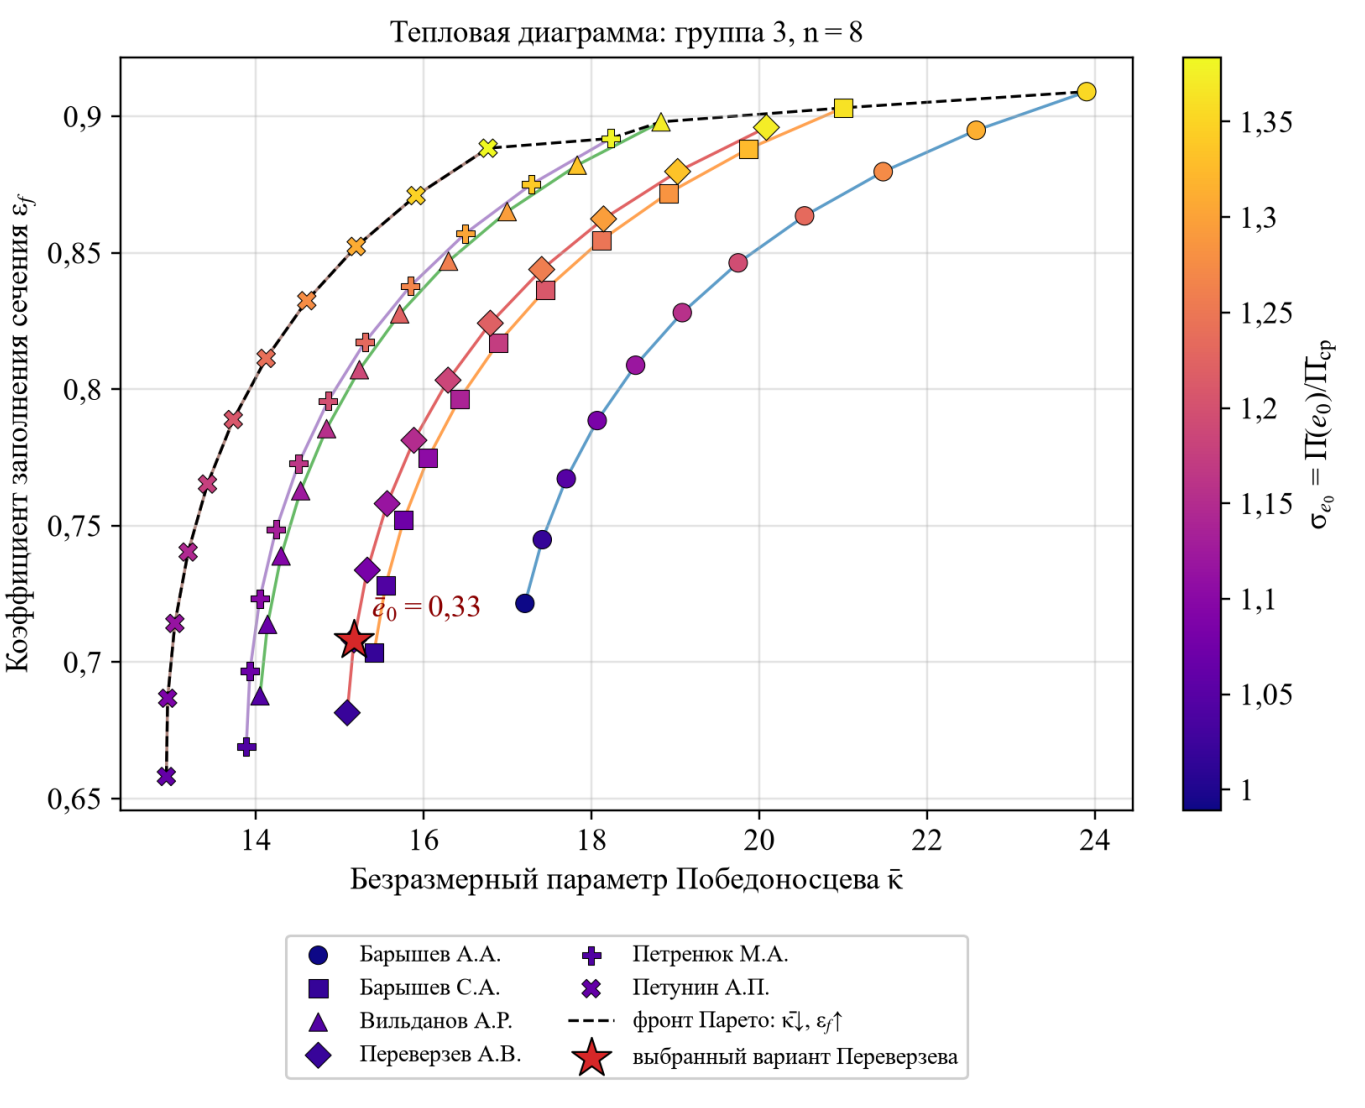
\includegraphics[width=0.84\textwidth]{thermal_diagram_group_reference.png}
          \figurecaption{Рисунок 1 — Общая тепловая диаграмма вариантов группы 3}
        \end{figure}
        На общей диаграмме круги соответствуют Барышеву А.А., квадраты — Барышеву С.А., треугольники — Вильданову А.Р., ромбы — Переверзеву А.В., знаки «плюс» — Петренюку М.А., кресты — Петунину А.П. Абсцисса характеризует риск эрозионного горения: меньшие значения $\bar\kappa_{\max}$ предпочтительнее. Ордината характеризует заполнение поперечного сечения: большее $\varepsilon_f$ предпочтительнее. Цвет точки определяет $\sigma_{e_0}$ и показывает отклонение площади горения от среднего значения на момент $e_0$. Пунктирная линия показывает фронт Парето; красная звезда на исходной групповой диаграмме отмечает выбранный вариант Переверзева А.В.
        На общей диаграмме рост $\bar e_0$ для каждого варианта даёт совместное увеличение $\varepsilon_f$ и $\bar\kappa_{\max}$: канал в начальный момент становится меньше, топливное заполнение повышается, но отношение периметра к площади свободного прохода возрастает. Следовательно, увеличение $\varepsilon_f$ является компромиссом: оно сопровождается ростом параметра Победоносцева. При выборе индивидуальной точки необходимо контролировать также $\sigma_{e_0}$: близость к единице означает малое отклонение площади горения от средней.

        На рисунке~\ref{fig:perimeter} приведена зависимость безразмерного периметра от толщины сгоревшего свода для индивидуального варианта Барышева С.А.: по 11 значениям $\bar e_0$ от 0,30 до 0,60. Тонкие вертикальные линии отмечают соответствующие значения $\bar e_0$ — границу между второй и третьей стадиями. После этой границы периметр снижается, что отражает догорание дегрессивных остатков.

        \begin{figure}[H]\centering
          \refstepcounter{figure}\label{fig:perimeter}
          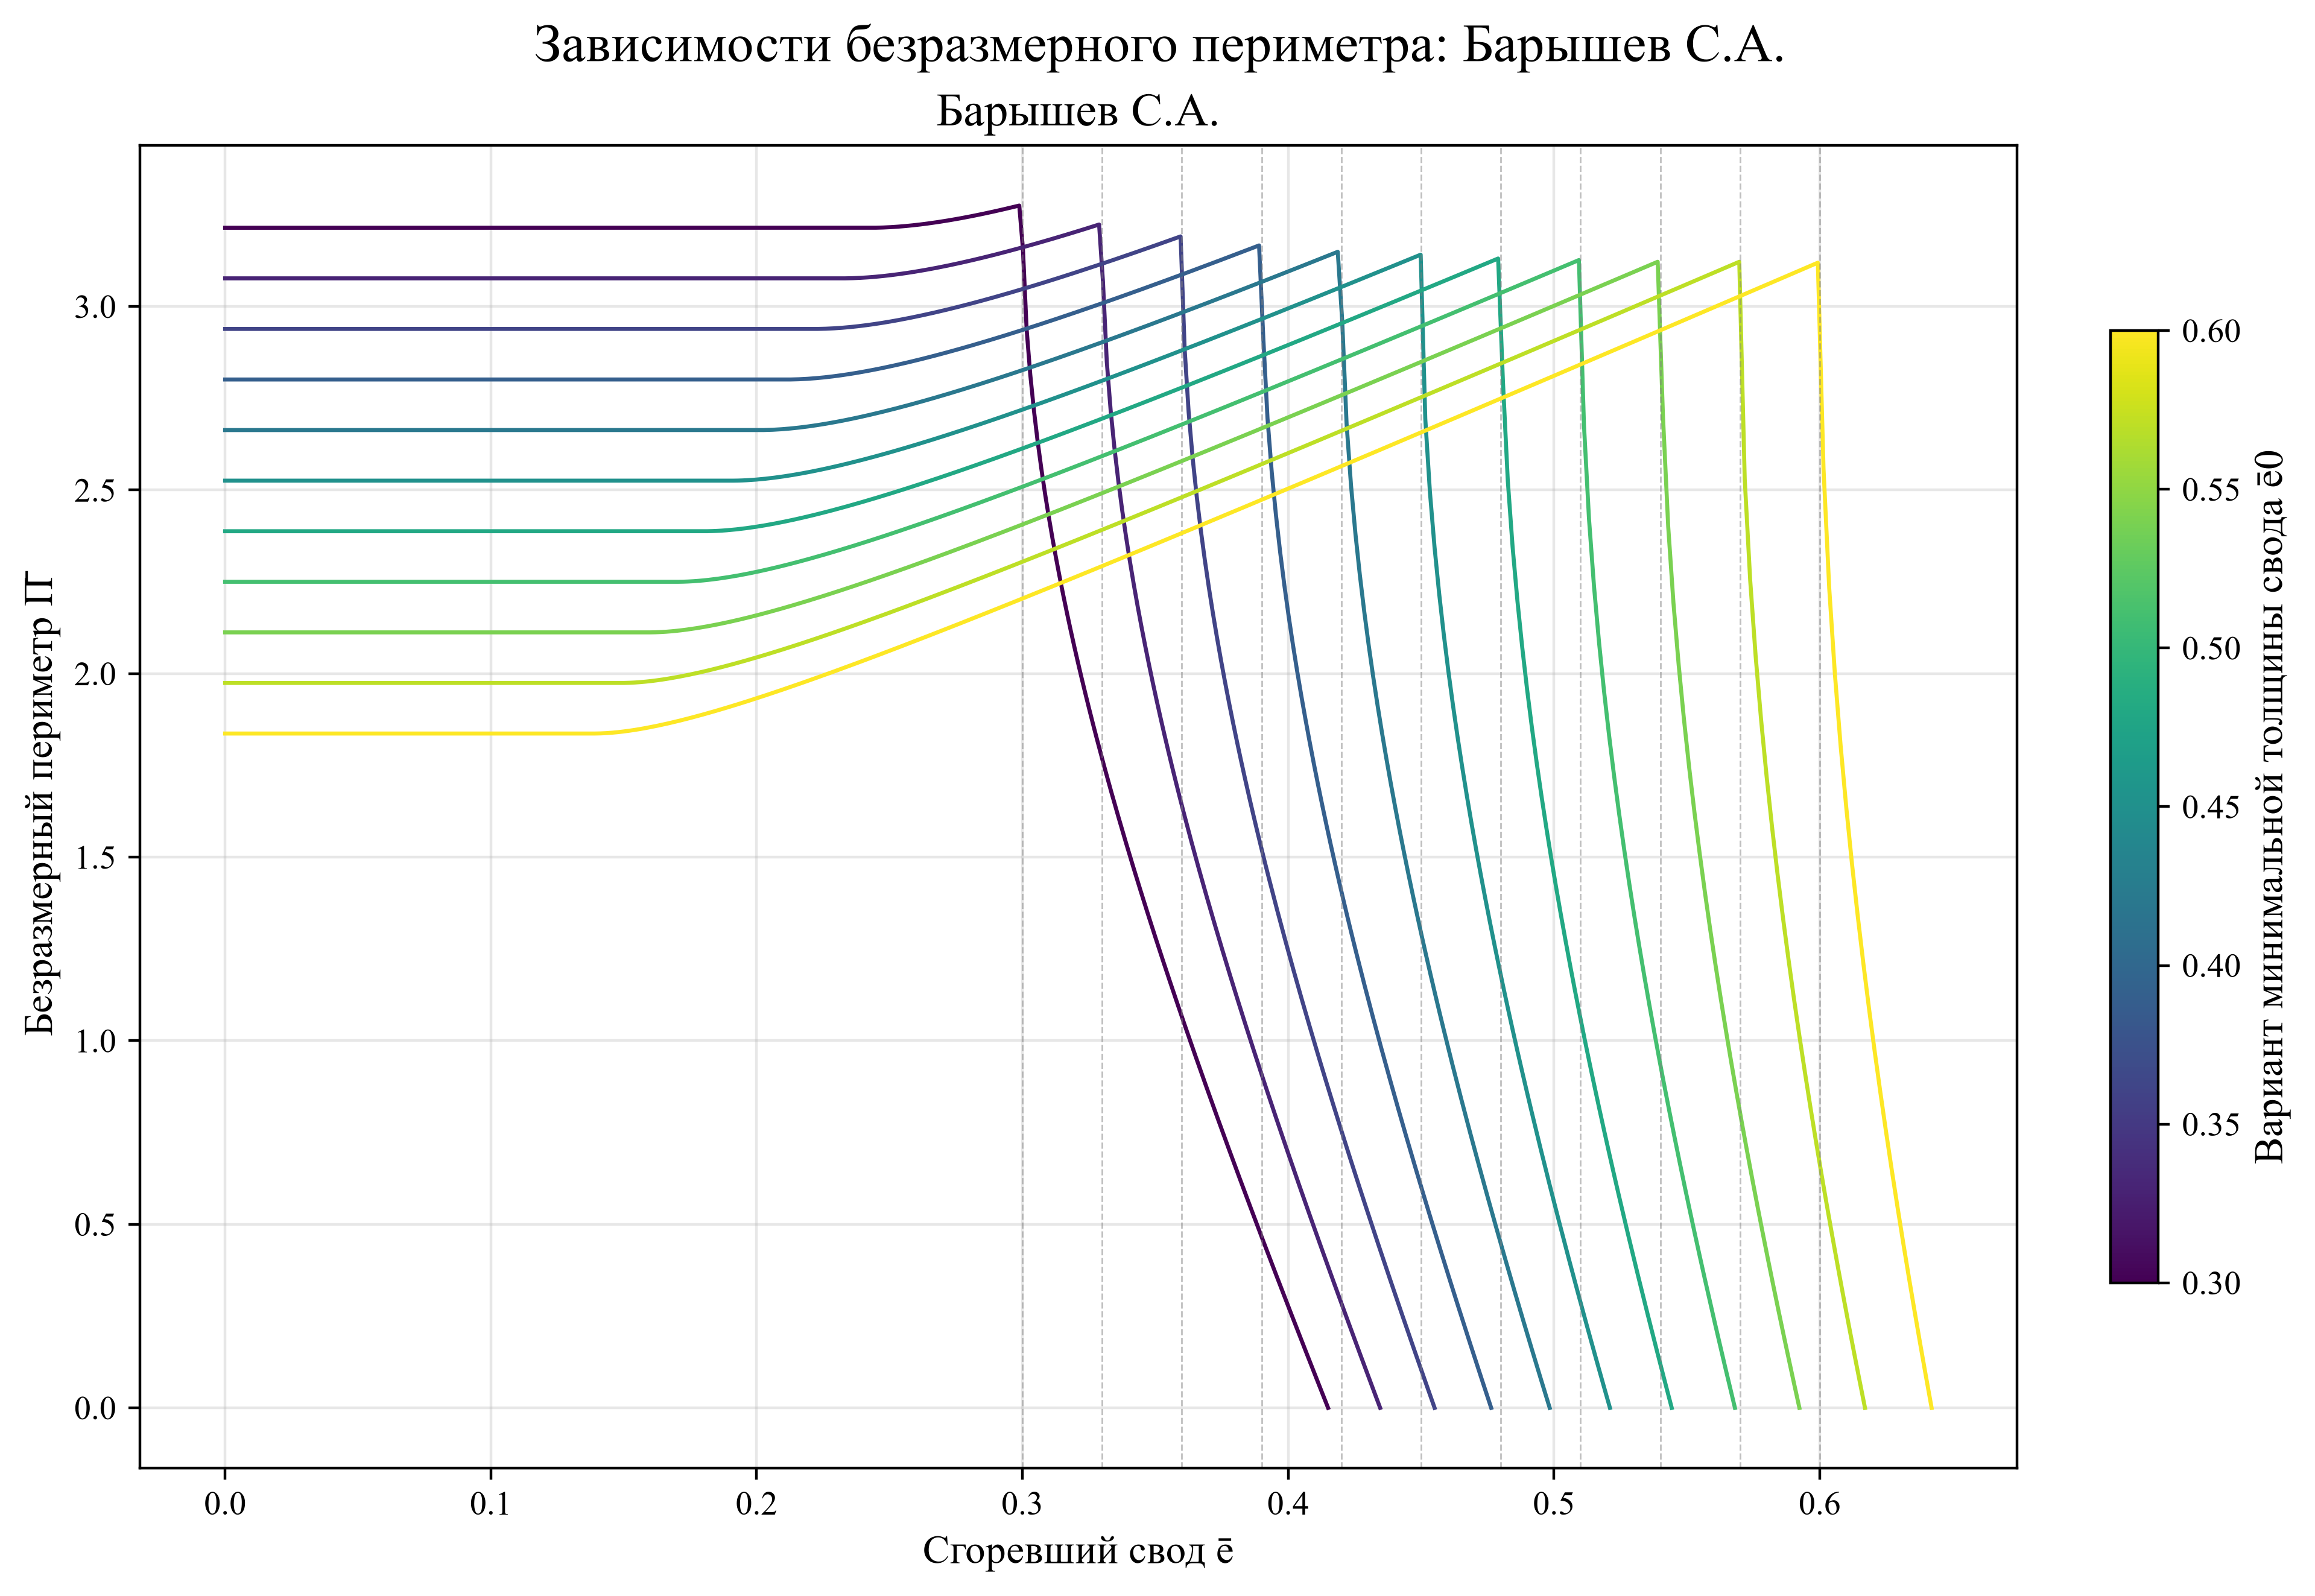
\includegraphics[width=0.88\textwidth]{perimeter_curves_baryshev_SA.png}
          \figurecaption{Рисунок 2 — Зависимость безразмерного периметра от толщины сгоревшего свода для индивидуального варианта Барышева С.А.}
        \end{figure}

        \clearpage
        Рисунок~\ref{fig:metrics} детализирует ход показателей индивидуального варианта Барышева С.А. С увеличением $\bar e_0$ коэффициент заполнения растёт от 0,7034 до 0,9031, одновременно растут $\bar\kappa_{\max}$ и отклонение $\sigma_{e_0}$ от единицы. Доля дегрессивных остатков, напротив, уменьшается от 0,1260 до 0,0317. Поэтому крайние значения $\bar e_0$ требуют компромисса: повышение заполнения сопровождается ростом параметра Победоносцева и более выраженной прогрессивностью процесса.

        \begin{figure}[H]\centering
          \refstepcounter{figure}\label{fig:metrics}
          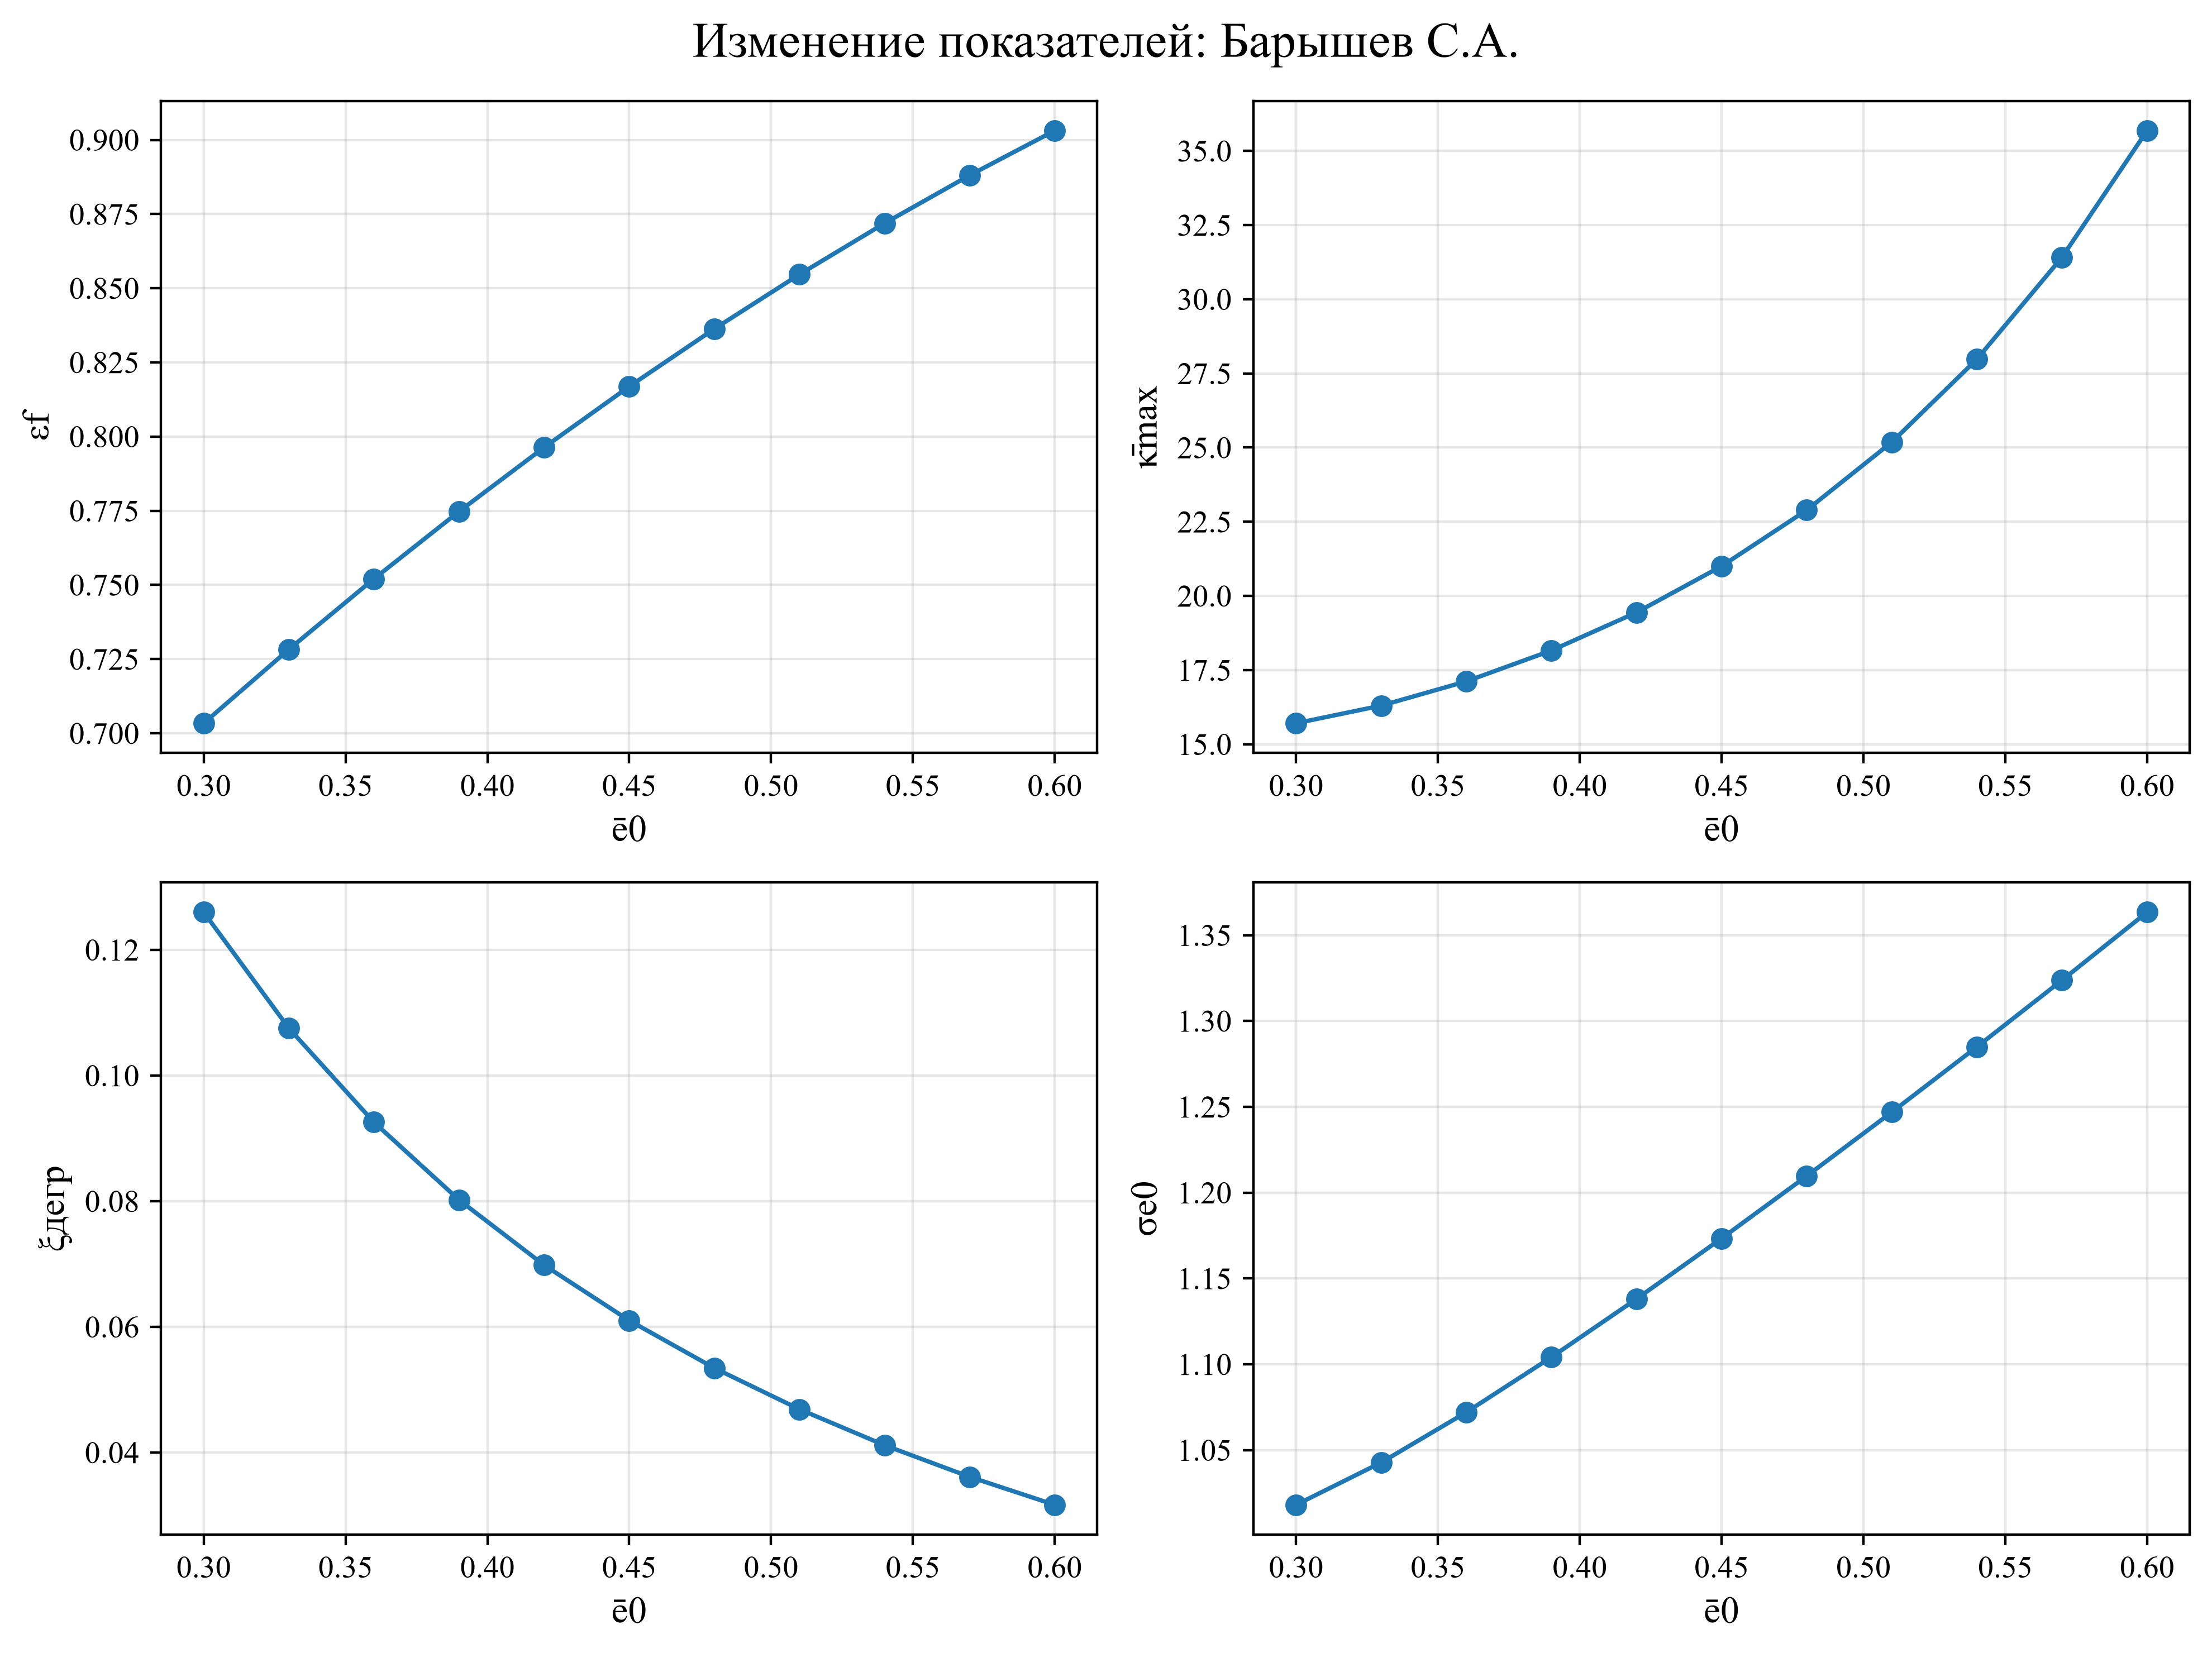
\includegraphics[width=0.88\textwidth]{individual_metrics_baryshev_SA.png}
          \figurecaption{Рисунок 3 — Изменение показателей индивидуального варианта Барышева С.А.}
        \end{figure}

        \clearpage
        \heading{5. Параметры для построения на миллиметровой бумаге}
        В отчёт не включается чертёж звезды на миллиметровой бумаге. Для его самостоятельного построения выбран разумный наружный диаметр $D=100$ мм. Для выбранного варианта $\bar e_0=0,330$ параметры рисунка 2 методических указаний имеют значения: $e_0=16,500$ мм, $R=30,455$ мм, $r=3,045$ мм, $\alpha=22,500^\circ$, $\beta=37,307^\circ$, $\gamma=75.193^\circ$. Дополнительно: длина плоской части луча в начальный момент $b(0)=15.233$ мм, граница первой стадии $e_1=11,607$ мм, конец горения дегрессивных остатков $e_{\max}=21,730$ мм. Эти данные следует зеркально отложить относительно оси полулуча и повторить для восьми лучей с шагом $45^\circ$.

        \clearpage
        \heading{6. Заключение}
        Для индивидуального варианта Барышева С.А. выбран $\bar e_0=0,33$. При нём $\varepsilon_f=0,7283$, $\bar\kappa_{\max}=16,301$, $\xi_{\mathrm{дегр}}=0,1075$, $\sigma_{e_0}=1,0427$. По сравнению с $\bar e_0=0,30$ коэффициент заполнения увеличивается с 0,7034 до 0,7283, а доля дегрессивных остатков уменьшается с 0,1260 до 0,1075. Рост $\bar\kappa_{\max}$ остаётся умеренным, а отклонение $\sigma_{e_0}$ от единицы составляет около 5\%, поэтому закон изменения поверхности горения близок к нейтральному. Варианты с большим $\bar e_0$ обеспечивают более высокое заполнение, но дают заметно больший максимум параметра Победоносцева и более выраженную прогрессивность, поэтому для выбранного варианта они менее рациональны.

        \end{document}
